% Options for packages loaded elsewhere
\PassOptionsToPackage{unicode}{hyperref}
\PassOptionsToPackage{hyphens}{url}
%
\documentclass[
]{article}
\usepackage{amsmath,amssymb}
\usepackage{iftex}
\ifPDFTeX
  \usepackage[T1]{fontenc}
  \usepackage[utf8]{inputenc}
  \usepackage{textcomp} % provide euro and other symbols
\else % if luatex or xetex
  \usepackage{unicode-math} % this also loads fontspec
  \defaultfontfeatures{Scale=MatchLowercase}
  \defaultfontfeatures[\rmfamily]{Ligatures=TeX,Scale=1}
\fi
\usepackage{lmodern}
\ifPDFTeX\else
  % xetex/luatex font selection
\fi
% Use upquote if available, for straight quotes in verbatim environments
\IfFileExists{upquote.sty}{\usepackage{upquote}}{}
\IfFileExists{microtype.sty}{% use microtype if available
  \usepackage[]{microtype}
  \UseMicrotypeSet[protrusion]{basicmath} % disable protrusion for tt fonts
}{}
\makeatletter
\@ifundefined{KOMAClassName}{% if non-KOMA class
  \IfFileExists{parskip.sty}{%
    \usepackage{parskip}
  }{% else
    \setlength{\parindent}{0pt}
    \setlength{\parskip}{6pt plus 2pt minus 1pt}}
}{% if KOMA class
  \KOMAoptions{parskip=half}}
\makeatother
\usepackage{xcolor}
\usepackage[margin=1in]{geometry}
\usepackage{graphicx}
\makeatletter
\def\maxwidth{\ifdim\Gin@nat@width>\linewidth\linewidth\else\Gin@nat@width\fi}
\def\maxheight{\ifdim\Gin@nat@height>\textheight\textheight\else\Gin@nat@height\fi}
\makeatother
% Scale images if necessary, so that they will not overflow the page
% margins by default, and it is still possible to overwrite the defaults
% using explicit options in \includegraphics[width, height, ...]{}
\setkeys{Gin}{width=\maxwidth,height=\maxheight,keepaspectratio}
% Set default figure placement to htbp
\makeatletter
\def\fps@figure{htbp}
\makeatother
\setlength{\emergencystretch}{3em} % prevent overfull lines
\providecommand{\tightlist}{%
  \setlength{\itemsep}{0pt}\setlength{\parskip}{0pt}}
\setcounter{secnumdepth}{-\maxdimen} % remove section numbering
\ifLuaTeX
  \usepackage{selnolig}  % disable illegal ligatures
\fi
\IfFileExists{bookmark.sty}{\usepackage{bookmark}}{\usepackage{hyperref}}
\IfFileExists{xurl.sty}{\usepackage{xurl}}{} % add URL line breaks if available
\urlstyle{same}
\hypersetup{
  pdftitle={Figures and Tables},
  pdfauthor={J.P. Meagher},
  hidelinks,
  pdfcreator={LaTeX via pandoc}}

\title{Figures and Tables}
\author{J.P. Meagher}
\date{2024-04-14}

\begin{document}
\maketitle

\hypertarget{background}{%
\section{Background}\label{background}}

\hypertarget{exploratory-analysis}{%
\subsection{Exploratory analysis}\label{exploratory-analysis}}

This section of the manuscript includes three figures exploring various
aspects of the \texttt{r/ireland} dataset.

\hypertarget{figure-1}{%
\subsubsection{Figure 1}\label{figure-1}}

This figure highlights the branching structure associated with a typical
sequence of discussions and the circadian rhythm associated with overall
activity on the subreddit.

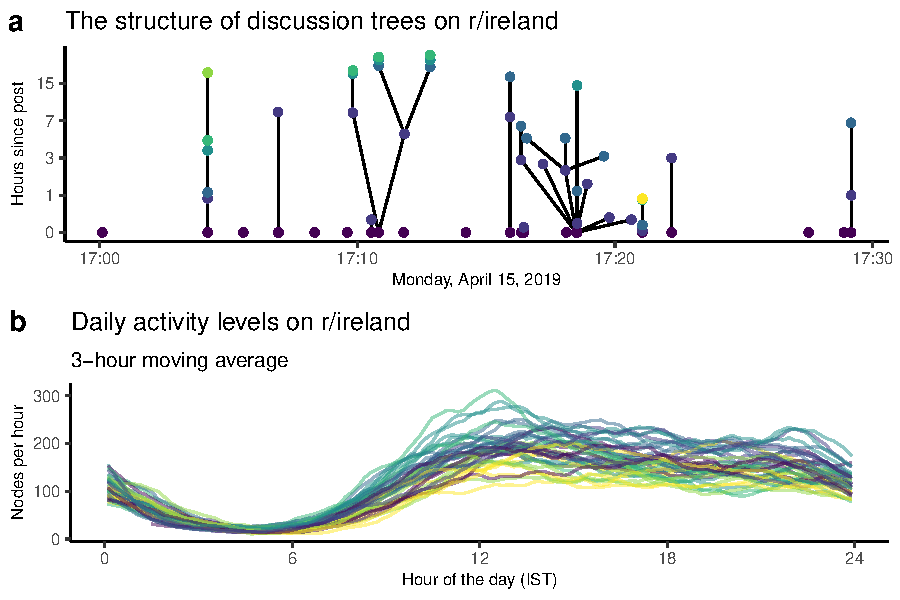
\includegraphics{figures_and_tables_files/figure-latex/data_exploration-1.pdf}

\hypertarget{figure-2}{%
\subsubsection{Figure 2}\label{figure-2}}

This figure highlights that the mean number of replies to each point
within the subreddit seems to follow a circadian rhythm and that the
distribution of the number of replies to each point is overdispersed
relative to the Poisson distribution.

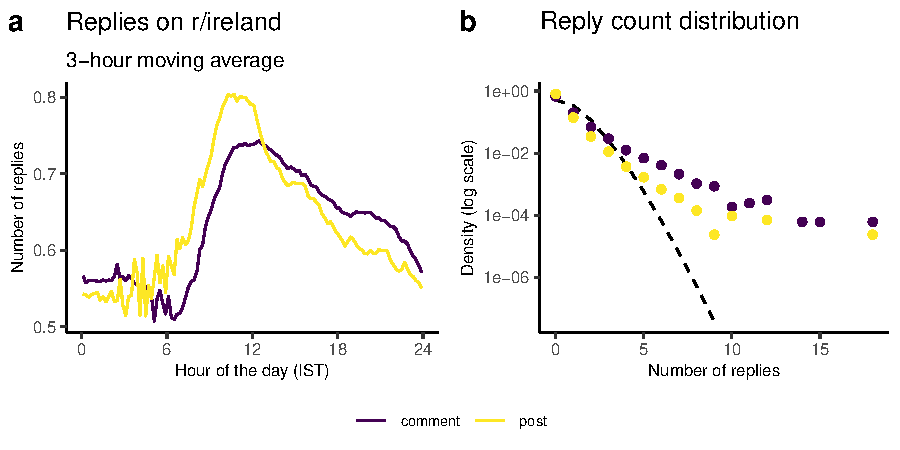
\includegraphics{figures_and_tables_files/figure-latex/reply_distribution_exploration-1.pdf}

\hypertarget{figure-3}{%
\subsubsection{Figure 3}\label{figure-3}}

The final figure in this section illustrates that the distribution of
generation intervals depends on the time of day that a point arrives.

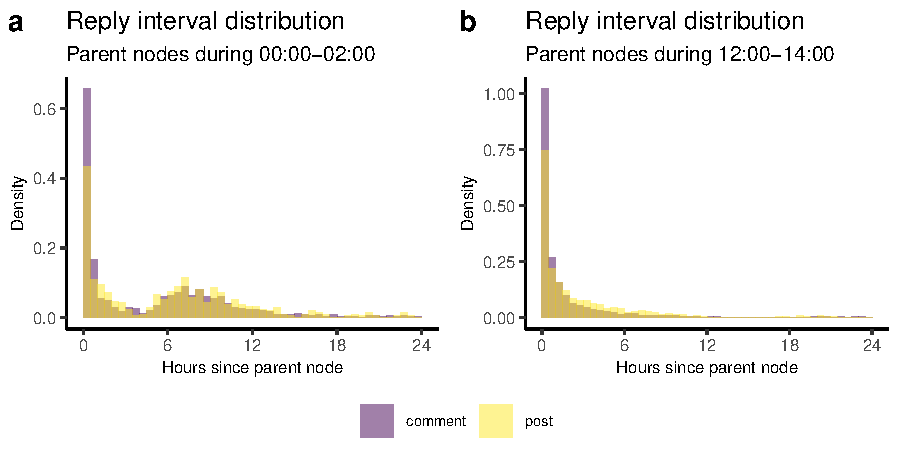
\includegraphics{figures_and_tables_files/figure-latex/reply_interval_exploration-1.pdf}

\hypertarget{methods}{%
\section{Methods}\label{methods}}

This section of the manuscript presents all the methods required to
conduct the reported analysis.

\hypertarget{the-generative-model}{%
\subsection{The generative model}\label{the-generative-model}}

\hypertarget{figure-4}{%
\subsubsection{Figure 4}\label{figure-4}}

This figure presents a synthetic cluster, highlighting relevant features
of the model. The figure consists of 4 elements.

First we present the simulated cluster illustrating individual
reproduction numbers and the branching structure.

The second element is the circadian rhythm modulating the overall
activity intensity.

The third element is the excitation induces by each new point given it's
individual reproduction number and the exponential excitation function.

The fourth and final element is the conditional intensity function
associated with the cluster.

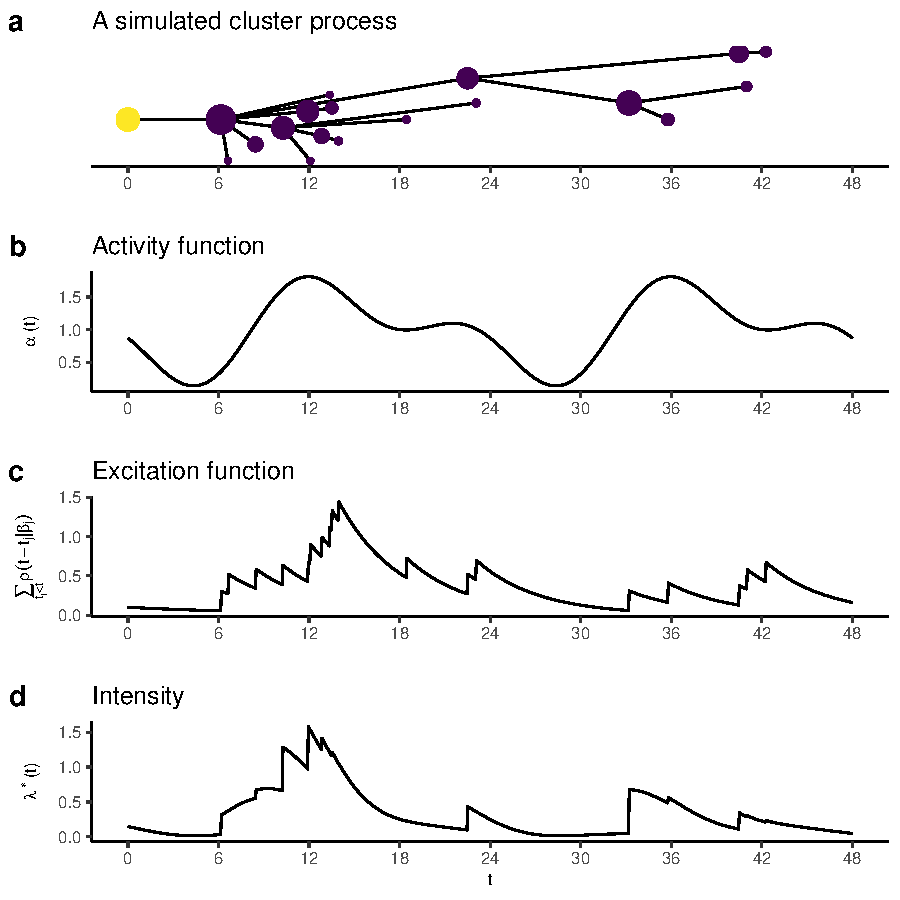
\includegraphics{figures_and_tables_files/figure-latex/model_form-1.pdf}

\hypertarget{results}{%
\section{Results}\label{results}}

This section of the manuscript presents the results of our analysis as a
series of tables and figures.

\hypertarget{inference}{%
\subsection{Inference}\label{inference}}

\hypertarget{table-2}{%
\subsubsection{Table 2}\label{table-2}}

This table summarises posterior distributions for each parameter of the
model relating to offspring processes.

\begin{table}[ht]
\centering
\begin{tabular}{|c|c|c|c|c|c|c|}
  \hline
Model & $\mu_1$ & $\mu_2$ & $\eta_1$ & $\eta_2$ & $\psi_1$ & $\psi_2$ \\ 
  \hline
$\mathcal M_1$ & 0.66 (0.01) & - & 0.33 (0.01) & - & - & - \\ 
  $\mathcal M_2$ & 0.65 (0.02) & 0.67 (0.01) & 0.27 (0.01) & 0.38 (0.01) & - & - \\ 
  $\mathcal M_3$ & 0.64 (0.02) & 0.64 (0.01) & 0.25 (0.01) & 0.34 (0.01) & - & - \\ 
  $\mathcal M_4$ & 0.65 (0.02) & 0.65 (0.01) & 0.25 (0.01) & 0.34 (0.01) & 1.15 (0.12) & 6.99 (1.63) \\ 
  $\mathcal M_5$ & 0.65 (0.02) & 0.64 (0.01) & 0.25 (0.01) & 0.34 (0.01) & 1.15 (0.12) & - \\ 
   \hline
\end{tabular}
\caption{Posterior mean (standard deviation) for the parameters $\boldsymbol \eta$, $\boldsymbol \mu$, and $\boldsymbol \psi$ within each of our candidate models. Considering each of the parameters in turn, the broad agreement on $\boldsymbol \mu$ across all the candidate models suggests that the expected number of offspring does not differ between immigrants and offspring. Differences in the offspring distributions for immigrants and offspring are manifest in the memory decay rate, which indicates that the expected generation interval for immigrants is longer than that for offspring. Finally, the values for $\boldsymbol \psi$ inferred by $\mathcal M_4$ suggest that immigrant points have a moderately heterogeneous offspring process while the offspring process for offspring is relatively homogeneous. As such, we include $\mathcal M_5$ in our analysis, which assumes heterogeneous immigrant and homogeneous offspring processes, respectively.} 
\label{tab:parameter_estimates}
\end{table}

We include calculations to support assertions on the posterior
distributions for each parameter included in the text.

\begin{verbatim}
##          mu[1] mu[2] eta[1] eta[2] psi[1] psi[2] inv_eta[1] inv_eta[2] tq[1]
## ci_lower  0.61  0.62   0.24   0.33   0.92   4.39       3.79       2.82  0.47
## ci_upper  0.70  0.68   0.26   0.35   1.40  10.15       4.21       3.05  0.53
##          tq[2] prop_zero[1] prop_zero[2]
## ci_lower  0.29         0.58         0.52
## ci_upper  0.34         0.62         0.55
\end{verbatim}

\hypertarget{figure-5}{%
\subsubsection{Figure 5}\label{figure-5}}

This table presents out posterior inference for the activity function
\(\alpha (t)\).

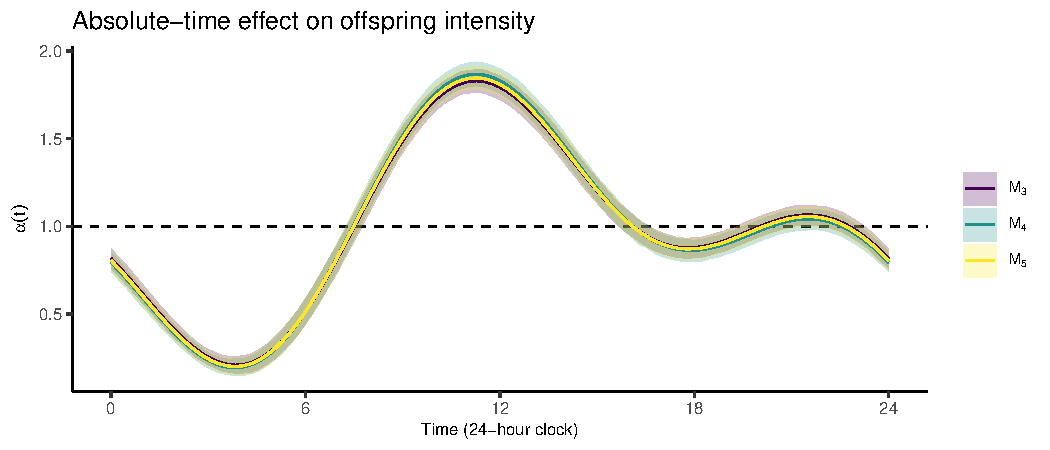
\includegraphics{figures_and_tables_files/figure-latex/alpha_inference-1.pdf}

\hypertarget{table-3}{%
\subsubsection{Table 3}\label{table-3}}

This table presents Bayes factors for each model, allowing us to assess
the evidence for each model.

\begin{table}[ht]
\centering
\begin{tabular}{|l|c|c|c|c|c|}
  \hline
 & $\mathcal {M}_1$ & $\mathcal {M}_2$ & $\mathcal {M}_3$ & $\mathcal {M}_4$ & $\mathcal {M}_5$ \\ 
  \hline
$\ln \mathcal{BF}_{l4}$ & -494.75 & -448.37 & -117.35 & 0.00 & -10.65 \\ 
   \hline
\end{tabular}
\caption{Estimated log Bayes factor for each candidate model relative to $\mathcal M_4$, that is, $\ln \mathcal{BF}_{l4}$ for $l = 1, \dots, 5$. Note that the evidence supporting each candidate model is estimated from the sampled posterior distribution $p \left( \theta \mid \boldsymbol y_{\operatorname{train}}, \mathcal M_l \right)$ via bridge sampling. In each case, the \texttt{bridgesampling} algorithm reports a coefficient of variation for the evidence estimate of $<0.005$, indicating that we have a precise estimate for each model evidence and, as a result, the corresponding Bayes factors. We find decisive evidence to support our inclusion of a circadian rhythm in the offspring intensity. Furthermore, we find decisive support for the inclusion of heterogeneous immigrant and offspring reproduction numbers.} 
\label{tab:bf_estimates}
\end{table}

We also check the Coefficient of variation associated with each model
evidence.

\begin{verbatim}
## [1] 0.0008276592
\end{verbatim}

\begin{verbatim}
## [1] 0.001166156
\end{verbatim}

\begin{verbatim}
## [1] 0.002134034
\end{verbatim}

\begin{verbatim}
## [1] 0.003607418
\end{verbatim}

\begin{verbatim}
## [1] 0.002648298
\end{verbatim}

\hypertarget{assessing-predictive-performance}{%
\subsection{Assessing Predictive
Performance}\label{assessing-predictive-performance}}

Here we assess the precictive performance of each model in terms of
expected predictive density and continuous ranked probability score.

\hypertarget{table-4}{%
\subsubsection{Table 4}\label{table-4}}

This table presents the expected log predictive density for each model,
allowing us to assess the predictive performance for each model.

\begin{table}[ht]
\centering
\begin{tabular}{|c|c|c|c|c|c|}
  \hline
 & $\mathcal {M}_1$ & $\mathcal {M}_2$ & $\mathcal {M}_3$ & $\mathcal {M}_4$ & $\mathcal {M}_5$ \\ 
  \hline
$\Delta \widehat{\operatorname{lpd}}_{l4}$ & -1004.6 (78.7) & -892.4 (71.8) & -177.5 (37.5) & 0.0 (0.0) & 17.2 (11.7) \\ 
   \hline
\end{tabular}
\caption{The difference (standard error) in log cluster-wise predictive density on $\boldsymbol y_{\operatorname{test}}$ between each model and $\mathcal M_4$. We find that $\mathcal M_4$ and $\mathcal M_5$ offer the best out-of-sample predictive performance in terms of $\operatorname{lpd}$, with $\mathcal M_5$ outperforming $\mathcal M_4$ slightly. This provides decisive support for the inclusion of a circadian rhythm and heterogeneous immigrant reproduction numbers in our model for online discussion on the \texttt{r/ireland} subreddit.} 
\label{tab:lpd}
\end{table}

\hypertarget{figure-6}{%
\subsubsection{Figure 6}\label{figure-6}}

This figure presents our analysis of the CRPS skill score comparing the
predictions for the cluster size after 48 hours to the empirical
distribution.

We start by computing the mean CRPS for the training set of clusters
using the empirical distribution.

Create the data frame required to present the CRPS skill scores for each
learning interval.

We then construct the plot illustrating skill scores.

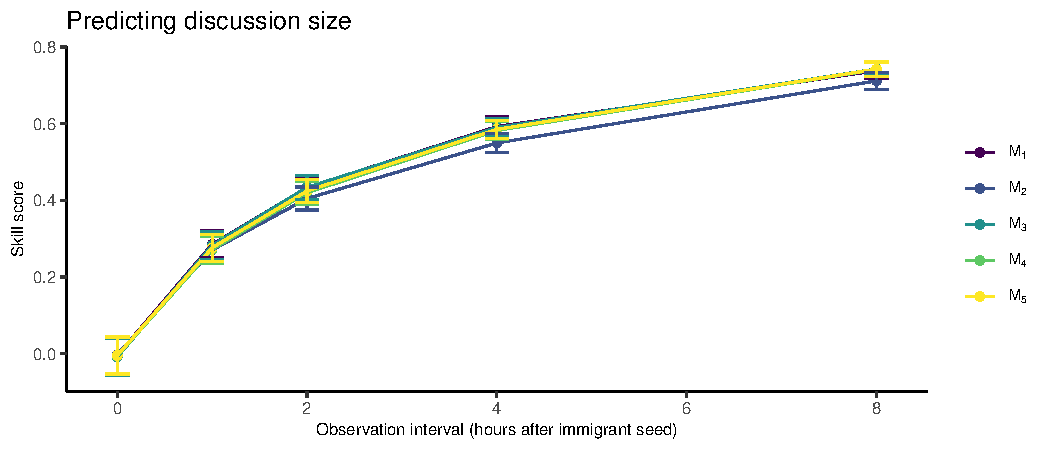
\includegraphics{figures_and_tables_files/figure-latex/crps_assessment-1.pdf}

\hypertarget{assessing-goodness-of-fit}{%
\subsection{Assessing goodness-of-fit}\label{assessing-goodness-of-fit}}

\hypertarget{figure-7}{%
\subsubsection{Figure 7}\label{figure-7}}

This figure present an analysis of the goodness of fit for each model to
the set of all discussions seeded during the training interval.

We first compute bootstrapped estimates of the ks test statistic
comparing predicted cluster sizes from each model to the empirical data.

We then compare the mean discussion size for each hour of the day using
only our full generative model and the empirical data.

Finally, we produce quantile-quantile plots comparing the distriution of
discussion sizes for each model to the empirical distribution

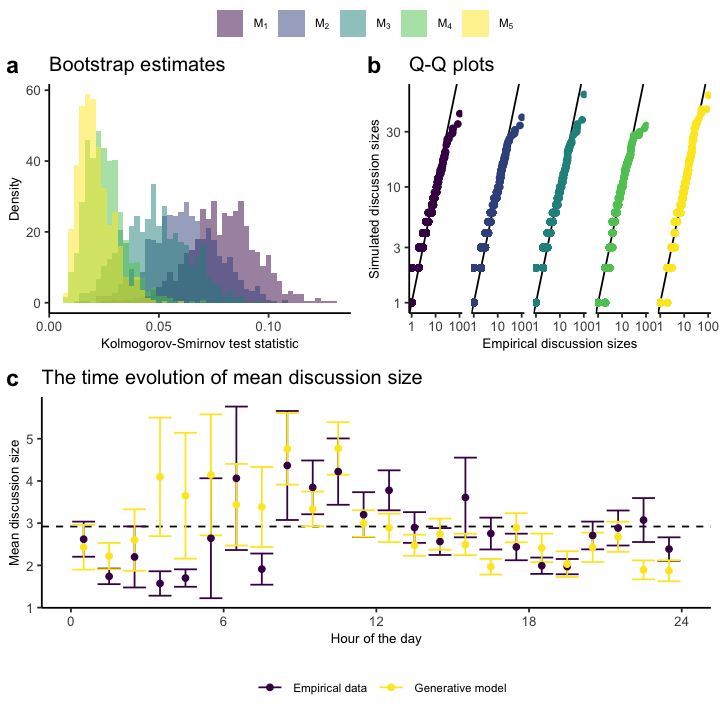
\includegraphics{figures_and_tables_files/figure-latex/gof-1.png}

\hypertarget{appendices}{%
\section{Appendices}\label{appendices}}

\hypertarget{circadian-rhythm}{%
\subsection{Circadian Rhythm}\label{circadian-rhythm}}

\hypertarget{figure-8}{%
\subsubsection{Figure 8}\label{figure-8}}

Perform the spectral analysis

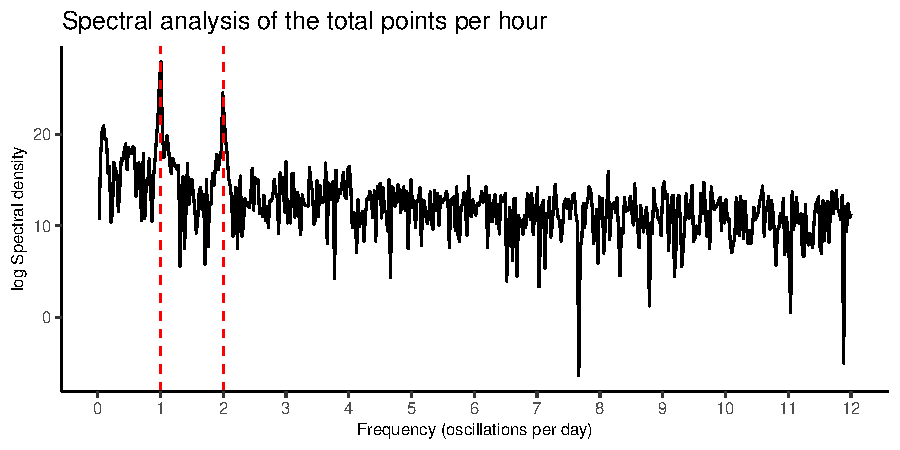
\includegraphics{figures_and_tables_files/figure-latex/count_spectral_density-1.pdf}

\hypertarget{table-5}{%
\subsubsection{Table 5}\label{table-5}}

Assess evidence for each basis function

\begin{table}[ht]
\centering
\begin{tabular}{|l|c|c|c|c|}
  \hline
 & $\mathcal {M}_1$ & $\mathcal {M}_2$ & $\mathcal {M}_3$ & $\mathcal {M}_4$ \\ 
  \hline
$\ln \mathcal{BF}_{l2}$ & -170.23 & 0.00 & 5.01 & 16.12 \\ 
   \hline
\end{tabular}
\caption{Estimated log Bayes factor for each candidate model relative to $\mathcal M_2$, that is, $\ln \mathcal{BF}_{l2}$ for $l = 1, \dots, 4$. The evidence supporting each candidate model is estimated from the sampled posterior distribution $p \left( \theta \mid \boldsymbol y_{\operatorname{train}}, \mathcal M_l \right)$ via bridge sampling. In each case, the \texttt{bridgesampling} algorithm reports a coefficient of variation for the evidence estimate of $<0.005$, indicating that we have a precise estimate for each model evidence. This analysis presents overwhelming evidence to support a choice of $K > 1$.} 
\label{tab:freq_bf_estimates}
\end{table}

\hypertarget{figure-9}{%
\subsubsection{Figure 9}\label{figure-9}}

Plot the activity function under each model

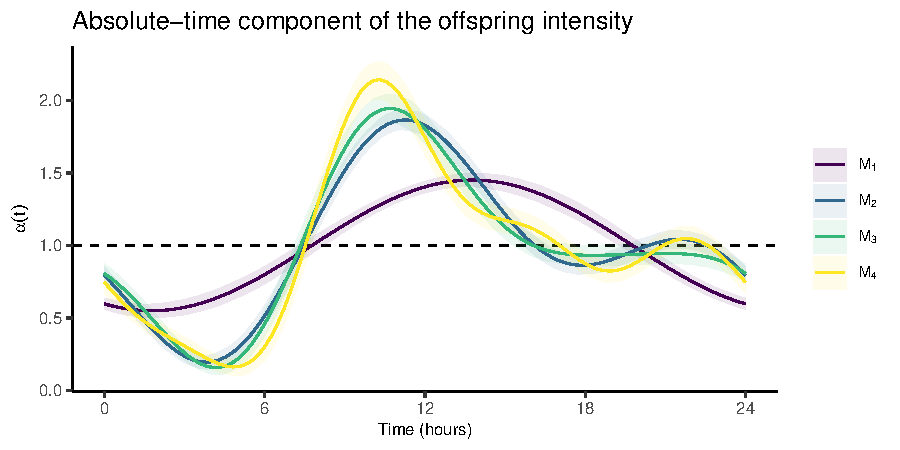
\includegraphics{figures_and_tables_files/figure-latex/freq_activity_functions-1.pdf}

\hypertarget{immigrant-arrivals}{%
\subsection{Immigrant arrivals}\label{immigrant-arrivals}}

\hypertarget{figure-10}{%
\subsubsection{Figure 10}\label{figure-10}}

Plot circadian activity functions for immigrant and offspring intensity
functions.

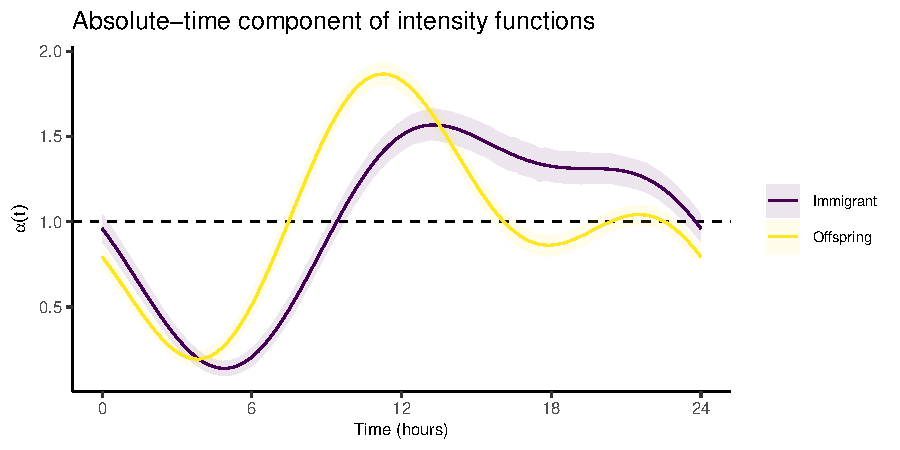
\includegraphics{figures_and_tables_files/figure-latex/immigrant_activity_function-1.pdf}

\end{document}
